\section{VM-centric Snapshot Deduplication}
\label{sect:deduplication}


With the considerations discussed in the previous section, we propose a
VM-centric approach (called VC)
for a co-located backup service that has a resource usage profile
suitable for use with converged cloud architectures.
This compares the traditional deduplication approach {\em VM-oblivious} (VO)
which manages duplicate data chunks without consideration of VMs.
Section~\ref{sect:vc-strategies} discusses  our key ideas and design for duplicate detection.
Section~\ref{sect:delete} presents  a simplified snapshot deletion with  the VM-centric approach.

\subsection{VM centric  strategies}
\label{sect:vc-strategies}

We describe our overall deduplication approach as consisting of three
complementary strategies: VM-local
duplicate search, global deduplication using popular chunks, and 
VM-centric file system block management. 
\begin{itemize}
\item 
\textbf{Cross-VM global deduplication using popular chunks} --
We separate the deduplication within a VM and cross VMs
and simplify the cross-VM deduplication while maximizing the inter-VM deduplication efficiency  as much as possible.
This is because global deduplication that detects the appearance of a chunk 
in any VM requires a substantial resource for fingerprint comparison.
To simplify cross-VM deduplication, we restrict the search scope of deduplication within the top $k$ most popular items.
%This step accomplishes the canonical global fingerprint lookup using a popular fingerprint index.
 \begin{figure}
 \centering
  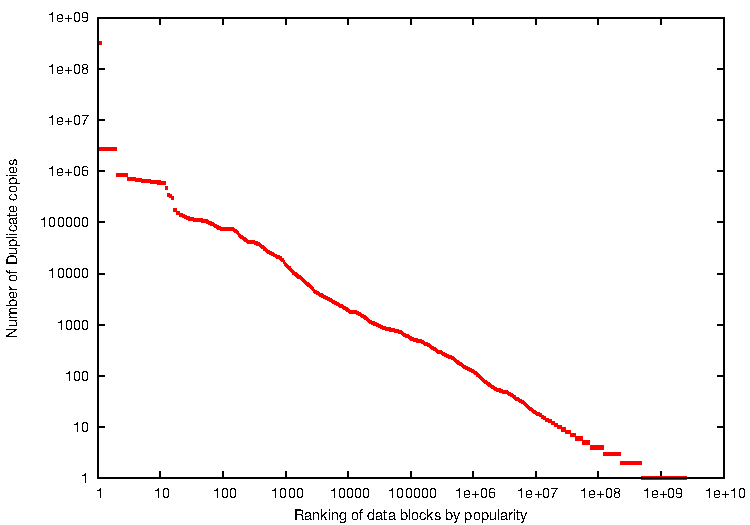
\includegraphics[width=2.5in]{figures/zipf_count_rank.pdf}
 \caption{Duplicate frequency versus  chunk ranking in a log scale after local deduplication.}
 \label{fig:Datazipf}
 \end{figure}


% {\it [Need to find a place to put these numbers in: Total number of chunks 
% in 350 snapshots: 1,546,635,485. 
% Total number of chunks after localized dedup: 283,121,924. Total number of unique chunks: 87,692,682.]}
Our key observation is for those chunks that appear in different VMs, top $k$ most popular items
dominate the distribution.  This popular data set is called the \textbf{PDS}. 
Figure~\ref{fig:Datazipf} shows the distribution of chunk popularity for a data trace 
from Alibaba with 2500 VMs discussed in Section ~\ref{sect:evaluation}.
We define chunk popularity as the number of unique copies of the chunk in the data-store,
i.e., the number of copies of the chunk after local deduplication.
%the distribution of chunk popularity~\cite{WeiZhangIEEE} 
%based on a production data trace from Alibaba with over 2500 VMs.
The distribution from this figure is Zipf-like. 
Let  $\sigma$ denote as the percentage of unique data chunks belonging to PDS and 
from the evaluation in Section~\ref{sect:evaluation}, we find that
$\sigma$ with about  2\% can deliver a fairly competitive deduplication efficiency.
%$\sigma$ with about  range of 2 to 4\% can deliver a fairly competitive deduplication efficiency.
%For example,
%with top 2\% of the most popular chunks stored in PDS, up-to 40\% of the raw backup 
%data can be eliminated by fingerprint lookup in PDS index.

%when restricting fingerprint comparison within a VM uses
%only a small amount of resource. 
%ehat the local deduplication has removed most of the duplicates.
%There are fewer deduplication opportunities across VMs while the memory and network
%consumption for global comparison is more expensive.
%Thus our approximation is that the global cross-VM fingerprint comparison only searches for the top $k$
%most popular items. 
PDS  can be computed periodically, e.g., on a monthly basis.
%Once the popularity of all data chunks is collected, the system only maintains the top $k$
%most popular chunk fingerprints (called \textbf{PDS index}) in a distributed shared memory.  
%These top chunks are shared among multiple VMs and  since $\sigma$ is relatively small, 
%we can afford to provide extra replicas for these popular chunk data to enhance the fault resilience.
%Compared to a preliminary solution which  uses data popularity~\cite{WeiZhangIEEE}, 
%this paper provides  a more comprehensive scheme with  improved deduplication efficiency and fault tolerance, and
%analytic design guidance. 

% Figure~\ref{fig:Datazipf} illustrates the distribution of chunk popularity based on a data trace from Alibaba with over 2500 VMs.
% The distribution is zipf like and popular chunks are dominating the large portion of data chunks.
% We denote $\sigma$ as the percentage of unique data chunks belonging to PDS and from the evaluation we find that
% $\sigma$ with a range of 1 to 4\% can deliver a fairly competitive deduplication efficiency.

Compared to ~\cite{bottleneck08}, the fingerprint index  size is reduced by $1-\sigma$
and the searchable fingerprint space  becomes very small under the popularity constraint.  
The fingerprint-guided distributed mapping in ~\cite{extreme_binning09,Dong2011} narrows
the search scope of each data chunk, but it does not reduce th total amount of searchable fingerprints
used for the entire deduplication. 
%In comparison we only focus on top popular chunks among VMs and this
%significantly reduces the total amount of  searchable fingerprints. 

\comments{
We have not adopted the index sampling in \cite{Guo2011} because its extension for
for a distributed architecture is difficult.  To use a distributed memory version of the sampled index, every deduplication 
request may access a remote machine for index lookup and the overall overhead of access latency for all requests
can be significant.
}
\item 
\textbf{VM-specific duplicate search optimization} --
While cross-VM deduplication is simplified, we intend to optimize the VM-specific deduplication 
as much as possible under a reasonable memory consumption
 to make up the loss of deduplication opportunities due to the cross-VM popularity constraint.

%Fingerprint lookup within a VM does not require a signficant  amount of memory resource.

We start with the standard version-based detection~\cite{Clements2009,Vrable2009}
to identify changed content with dirty bits in a coarse grain segment level.
%In our implementation 
%the segment size is 2MB
%and the device driver is extended to support tracking changed segments using a dirty bitmap. 
The reason to choose a coarse grain segment level is that 
since every write for a segment will touch a dirty bit, the device driver maintains dirty bits in 
memory and cannot afford a small segment size.
It should be noted that dirty bit tracking is supported or can be easily implemented in 
major virtualization solution vendors. 
%% this method is so widely-used and easy to understand, everyone include Pure Storage has it, I feel no need to explain further.
%{
%For example,
%the VMWare hypervisor has an API to let external backup applications know 
%the changed areas since last backup. 
%The Microsoft SDK provides an API that allows external applications to monitor 
%the VM's I/O traffic and implement such changed block tracking feature.
%}

\begin{figure}[htbp]
  \centering
  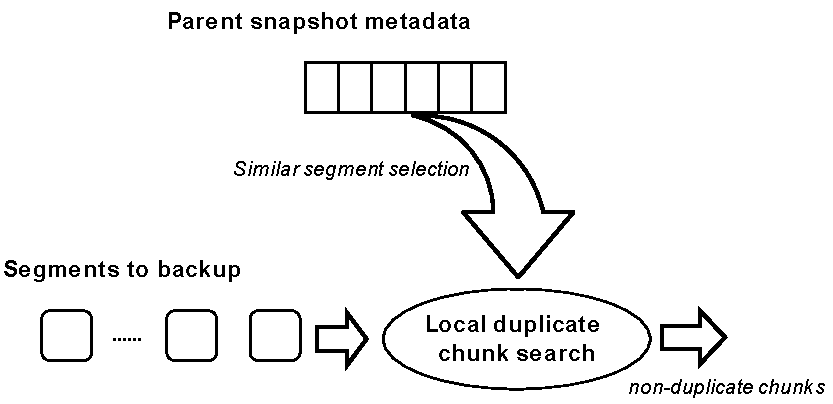
\epsfig{file=images/mh_local_dedup.pdf, width=2.7in}
  \caption{Similarity-guided local duplicate detection}
  \label{fig:local_dedup}
\end{figure}

Since the previous work typically uses a non-uniform chunk size 
with an average of 4KB or 8KB for the best deduplication 
effectiveness~\cite{Guo2011,extreme_binning09,bottleneck08,Dong2011},
we conduct additional local similarity guided deduplication on a snapshot by comparing
chunk fingerprints of a dirty segment 
with those in  {\em potentially similar} segments from its parent snapshot. 
We define a parent  segment is  potentially similar to the current segment if 1) the parent segment
at the same offset as the current segment.
2) the signature of these segments is the same.
This segment content signature value is defined as the minimum value of all its chunk fingerprints 
computed during backup and is recorded in the snapshot metadata (called recipe). 
%Note that this definition of content similarity is an approximation~\cite{resemblance97}.  
When processing a dirty segment,
its  similar segments can be found easily from the
parent snapshot recipe.  Then recipes of the similar segments are loaded to memory,
which contain chunk fingerprints to be compared.
To control the time cost of search, we set a limit on the number of  similar segment recipes to be fetched. 
% Then,
%given a set of data chunks within a dirty segment,  we compare  these chunk fingerprints
%with those in similar segments.  
For example, assume that  a segment is of size  2MB, 
its segment recipe is roughly 19KB which contains about 500 chunk fingerprints and other chunk metadata.
By limiting at most 10 similar segments to search, the amount of memory for maintaining those 
similar segment recipes is 190K, which is small.

%As part of our local duplicate search we also compare the current segment
%against the parent segment at the same offset.

\item 
\textbf{VM-centric file system block management} --
When a chunk is not detected as a duplicate to any existing chunk, this chunk will be written
into a file system block.  A  backend file system block can contain a number of chunks,
there are   two reasons. In addition to the reason that a file system block is often
configured to be large, there is another reason that a number of chunks can be combined together
and compressed further using a standard data compression method. 
%We manage this accumulation process using a log-structured storage scheme built
%on a distributed file system discussed in Section~\ref{sect:architecture}.
%Non-PDS chunks from the same VM are stored in one append store. 
We set two constraints in composing chunks for a file system block as follows:
1) Each file system block is either dedicated to non-PDS chunks, or PDS-chunks.
2) A non-PDS file system block is only associated with one VM.

Restricting the association with one VM improves fault isolation when some file blocks are lost during failure. 
In addition, storing PDS chunks separately allows special replication handling for those popular shared data. 
%%% talk something about snapshot store advantage here? %%%
%One could try to rely on filesystem features to 
If we do not separate the
popular chunks from the less-popular, the popular chunks are dispersed across
all of the filesystem blocks in the storage system and we would have
to add extra replications for {\em all} file blocks in order to   follow the popularity-driven replication idea 
from ~\cite{Reliability06}. That reduces the storage efficiency.
%Then we cannot leverage the file system features to 
%provide extra replication to popular and shared chunks because  
%we have to add extra replication to each file block as long as it contains a popular chunk.

%factor on popular chunks. This explains why we must separate the PDS and
%non-PDS data in our system to achieve the desired $r_c/r$ ratio (though both
%can be stored on the same DFS).

%The system allows all machines conduct backups in parallel, and each machine
%conducts the backup of one VM at a time, and thus only requires a write buffer for one VM.
\end{itemize}


